\documentclass{article} %article 文档
\usepackage{ctex}  %使用宏包(为了能够显示汉字)
\usepackage{graphicx} %图片控制宏包
\title{文章的标题}  %文章标题
\author{作者名称}   %作者的名称
\date{\today}       %日期
% 设置页面的环境,a4纸张大小,左右上下边距信息
\usepackage[a4paper,left=10mm,right=10mm,top=15mm,bottom=15mm]{geometry}


\begin{document}
% 1. 添加这一句才能够显示标题等信息
\maketitle

% 2. 摘要开始部分
\begin{abstract}
    该部分内容是放置摘要信息的。该部分内容是放置摘要信息的。该部分内容是放置摘要信息的。该部分内容是放置摘要信息的。该部分内容是放置摘要信息的。
\end{abstract}
% 3. 如果不希望摘要与正文在一页的话,在摘要结束后添加\newpage即可。
% \newpage

% 4. 标题开始
% 正文的标题设置:一级标题\section{},二级标题\subsection{},三级标题\subsubsection{};
% 正文的段落设置:在一段的最后添加\par代表一段的结束;
% 正文的目录设置:在\begin{document} 内容中添加:\tableofcontents

\section{一级标题1}
第一段一级标题下的内容,一级标题下的内容,一级标题下的内容,一级标题下的内容,一级标题下的内容,一级标题下的内容,一级标题下的内容,一级标题下的内容。。\par
第二段一级标题下的内容,一级标题下的内容,一级标题下的内容,一级标题下的内容,一级标题下的内容,一级标题下的内容,一级标题下的内容,一级标题下的内容。。
\subsection{二级标题1.1}
二级标题下的内容。。。
\subsubsection{三级标题下的内容1.1.1}
三级标题下的内容。。。
\section{一级标题2}
一级标题2中的内容\par


% 5. 脚注的使用:在需要添加脚注的文字后添加\footnote{脚注内容}即可;
% 引用的使用:\begin{quote}即可
% 字体的改变:使用{\fangsong } ,{}中的内容即为仿宋字体等。
西游记\footnote{中国古典四大名著之一}小说开头写道:
\begin{quote}
{\kaishu 东胜神洲有一花果山,山顶一石,受日月精华,生出一石猴。之后因为成功闯入水帘洞,被花果山诸猴拜为“美猴王”。}
\end{quote}

% 6. 图片的插入
% 需要使用宏包\usepackage{graphicx} %图片控制宏包;使用\caption{} 为图片添加名称。本图片已经放置在当前文件下。
%开始插入图片
\begin{figure}[htbp] %htbp 代表图片插入位置的设置
\centering %图片居中
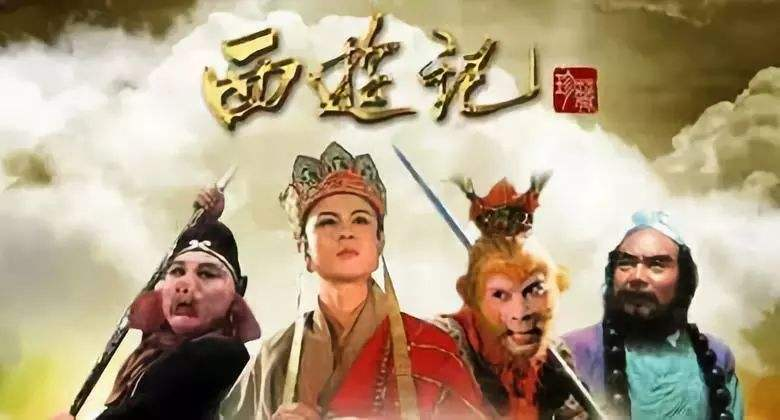
\includegraphics[width=5cm]{images/xiyouji.jpeg}%[]中可选参数,可以设置图片的宽高
%添加图体
\caption{六小龄童}
\label{fig:xiyouji}
\end{figure}

% 7. 表格插入
\begin{table}[htbp] %htbp代表表格浮动位置
%表格居中
\centering
%添加表头
\caption{西游记四人身份表}
%创建table环境
\begin{tabular}{cccc} %4个c代表4列都居中,也可以设置l,r
%表格的输入
\hline  %一条水平线
唐僧 & 孙悟空 &猪悟能 &沙悟净\\ %\\为换行符
\hline
唐玄奘 &美猴王 &天蓬元帅&卷帘大将\\
\hline
\end{tabular}
\end{table}

% 8. 数学符号的使用
% 行内公式用两个$包裹就行。行之间的公式,列表公式,使用\begin{equation}进行编写。(注意:在书写公示的时候,不应有空白行)

\section{函数,公式}
$\sin(x)$在数学中是三角函数中的一种,即为正弦函数.
\begin{equation}
y=\sin(x)
\end{equation}

% 9. 交叉引用
% 例如引用图片,在图片的名称(caption)后添加label{}标签,需要引用的部分使用?????? ,{}中填写label{}中的内容即可:
\section{交叉引用}
从图\ref{fig:fourp}中,可以看到师徒四人。
\begin{figure}[htbp]
\centering
% 
\includegraphics[width=\linewidth]{images/latex.png}
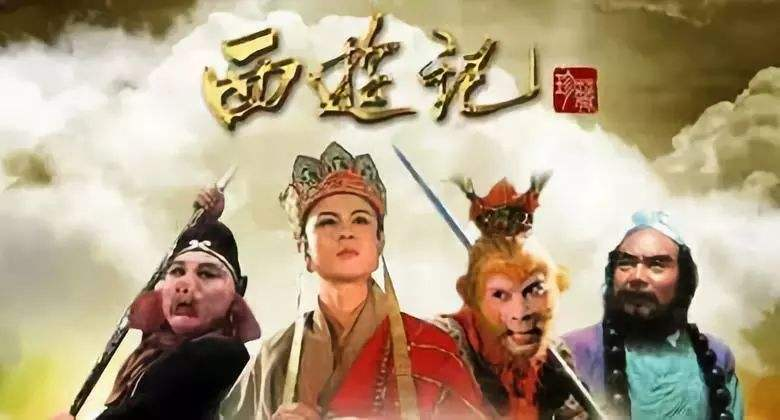
\includegraphics[height=10cm]{images/xiyouji.jpeg}
\caption{师徒四人}
\label{fig:fourp}
\end{figure}

Copy From: https://blog.csdn.net/meiqi0538/article/details/82887300

\end{document}
